\documentclass{beamer}
\usepackage{geometry}
\usepackage[english]{babel}
\usepackage[utf8]{inputenc}
\usepackage{amsmath}
\usepackage{amsfonts}
\usepackage{amssymb}
\usepackage{tikz}
\usetikzlibrary{quotes, angles}
\usepackage{graphicx}

%\usepackage{pgfplots}
%\pgfplotsset{width=10cm,compat=1.9}
%\usepackage{pgfplotstable}

\usepackage{fancyhdr}
\pagestyle{fancy}
\setlength{\headheight}{12pt}%doesn't seem to fix warning
\fancyhf{}

%\rhead{\small{10 September 2018}}
\lhead{\small{BECA / Dr. Huson / Geometry Unit 6: Analytic Geometry}}

\renewcommand{\headrulewidth}{0pt}

\title{Mathematics Class Slides}
\subtitle{Bronx Early College Academy}
\author{Chris Huson}
\date{25 November 2019}

\begin{document}
\frame{\titlepage}
\section[Outline]{}
\frame{\tableofcontents}

\section{6.1 Intro to the coordinate plane and linear functions, 25 November}
  \frame
  {
    \frametitle{GQ: How do we plot lines on the coordinate plane?}
    \framesubtitle{CCSS: HSG.GPE Express geometric properties with equations \hfill \alert{6.1 Monday 25 Nov}}

    \begin{block}{Do Now: Plotting points and lines}
    \begin{enumerate}
      \item Modeling geometric situations with an algebraic equation
      \item Slope-intercept form of linear equations
      \item Dilation of a line centered at the origin
    \end{enumerate}
    \end{block}
    Review exam results \\
    Lesson: Perpendicular and parallel slopes \\*[5pt]
    Homework: Test corrections due \alert{tomorrow}
  }

\section{6.2 Laptop practice - Geogebra graphing functions on coordinate plane, 26 November}
\frame
{
\frametitle{GQ: How do we work on the coordinate plane?}
\framesubtitle{CCSS: HSG.GPE Express geometric properties with equations \hfill \alert{6.2 Tuesday 26 Nov}}

\begin{block}{Do Now: Deltamath practice}
\begin{enumerate}
  \item Graphing linear equations
  \item Perpendicular and parallel slopes
  \item Function and algebraic manipulations
\end{enumerate}
\end{block}
10.1 meets in Room 414 first period tomorrow (advisory schedule)\\[0.5cm]
Homework: Complete Deltamath homework section
}

\section{6.3 Coordinate geometry practice, 27 November}
  \frame
  {
    \frametitle{GQ: How do we plot lines on the coordinate plane?}
    \framesubtitle{CCSS: HSG.GPE Express geometric properties with equations \hfill \alert{6.3 Wednesday 27 Nov}}

    \begin{block}{Do Now: Plotting points and lines}
    \begin{enumerate}
      \item Modeling geometric situations with an algebraic equation
      \item Slope-intercept form of linear equations
      \item Dilation of a line centered at the origin
    \end{enumerate}
    \end{block}
    Review exam results \\
    Lesson: Perpendicular and parallel slopes \\*[5pt]
    Homework: Test corrections due \alert{tomorrow}
  }

  \section{6.4 Assessment: distance formula, Monday 2 December}
  \frame
  {
    \frametitle{GQ: How do we plot lines on the coordinate plane?}
    \framesubtitle{CCSS: HSG.GPE Express geometric properties with equations \hfill \alert{6.4 Monday 2 Dec}}

    \begin{block}{Do Now: Plotting, measuring, and translating on the $x$-$y$ plane}
    \begin{enumerate}
      \item Measure horizontal and vertical distances
      \item Measure diagonal distances
      \item Parabolas, quadratic functions, \& function translation
    \end{enumerate}
    \end{block}
    Lesson: the distance formula (Pythagorean theorem)\\
    Review perpendicular and parallel slopes  \\*[5pt]
    Homework: Khan Academy distance practice
  }

  \section{6.4 Assessment: distance formula, Monday 2 December}
  \frame
  {
    \frametitle{Assessment: Distance formula (on looseleaf paper)}
    %\framesubtitle{CCSS: HSG.GPE Express geometric properties with equations \hfill \alert{6.4 Monday 2 Dec}}
    \begin{enumerate}
      \item Given $A(7,5)$ and $B(7,-4)$, find $AB$. \hspace{0.5cm}
        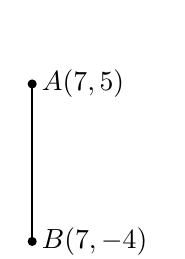
\begin{tikzpicture}[scale=1]
          \draw [thick] (0, 0)--(0,2);
          \draw [fill] (0,2) circle [radius=0.05] node[right]{$A(7,5)$};
          \draw [fill] (0,0) circle [radius=0.05] node[right]{$B(7,-4)$};
        \end{tikzpicture}\vspace{0.5cm}
      \item 
        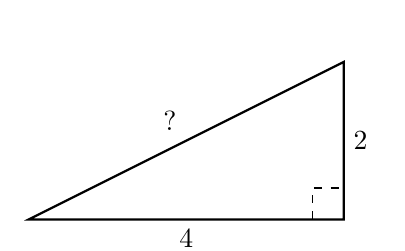
\begin{tikzpicture}[scale=1]
          \node at (2,1)[above left]{?};
          \node at (4,1)[right]{2};
          \node at (2,0)[below]{4};
          \draw [thick] (0, 0)--(4, 0)--(4, 2)--cycle;
          \draw [dashed] (4,0)++(-0.4,0)-- ++(0,0.4)-- +(0.4,0);
        \end{tikzpicture}
      \item What is the length of $\overline{CD}$ if $C(1,-2)$ and $D(7,6)$?
    \end{enumerate}
  }

  \section{6.5 Laptop practice - Geogebra distance and the Pythagorean theorem, 3 December}
  \frame
  {
  \frametitle{GQ: How do we calculate distance given coordinates?}
  \framesubtitle{CCSS: HSG.GPE Express geometric properties with equations \hfill \alert{6.5 Tuesday 3 Dec}}
  
  Do Now Assessment
  \begin{block}{Project paper: Use paper \& pencil or MS Word \& Geogebra}
  \begin{enumerate}
    \item Radical spiral
    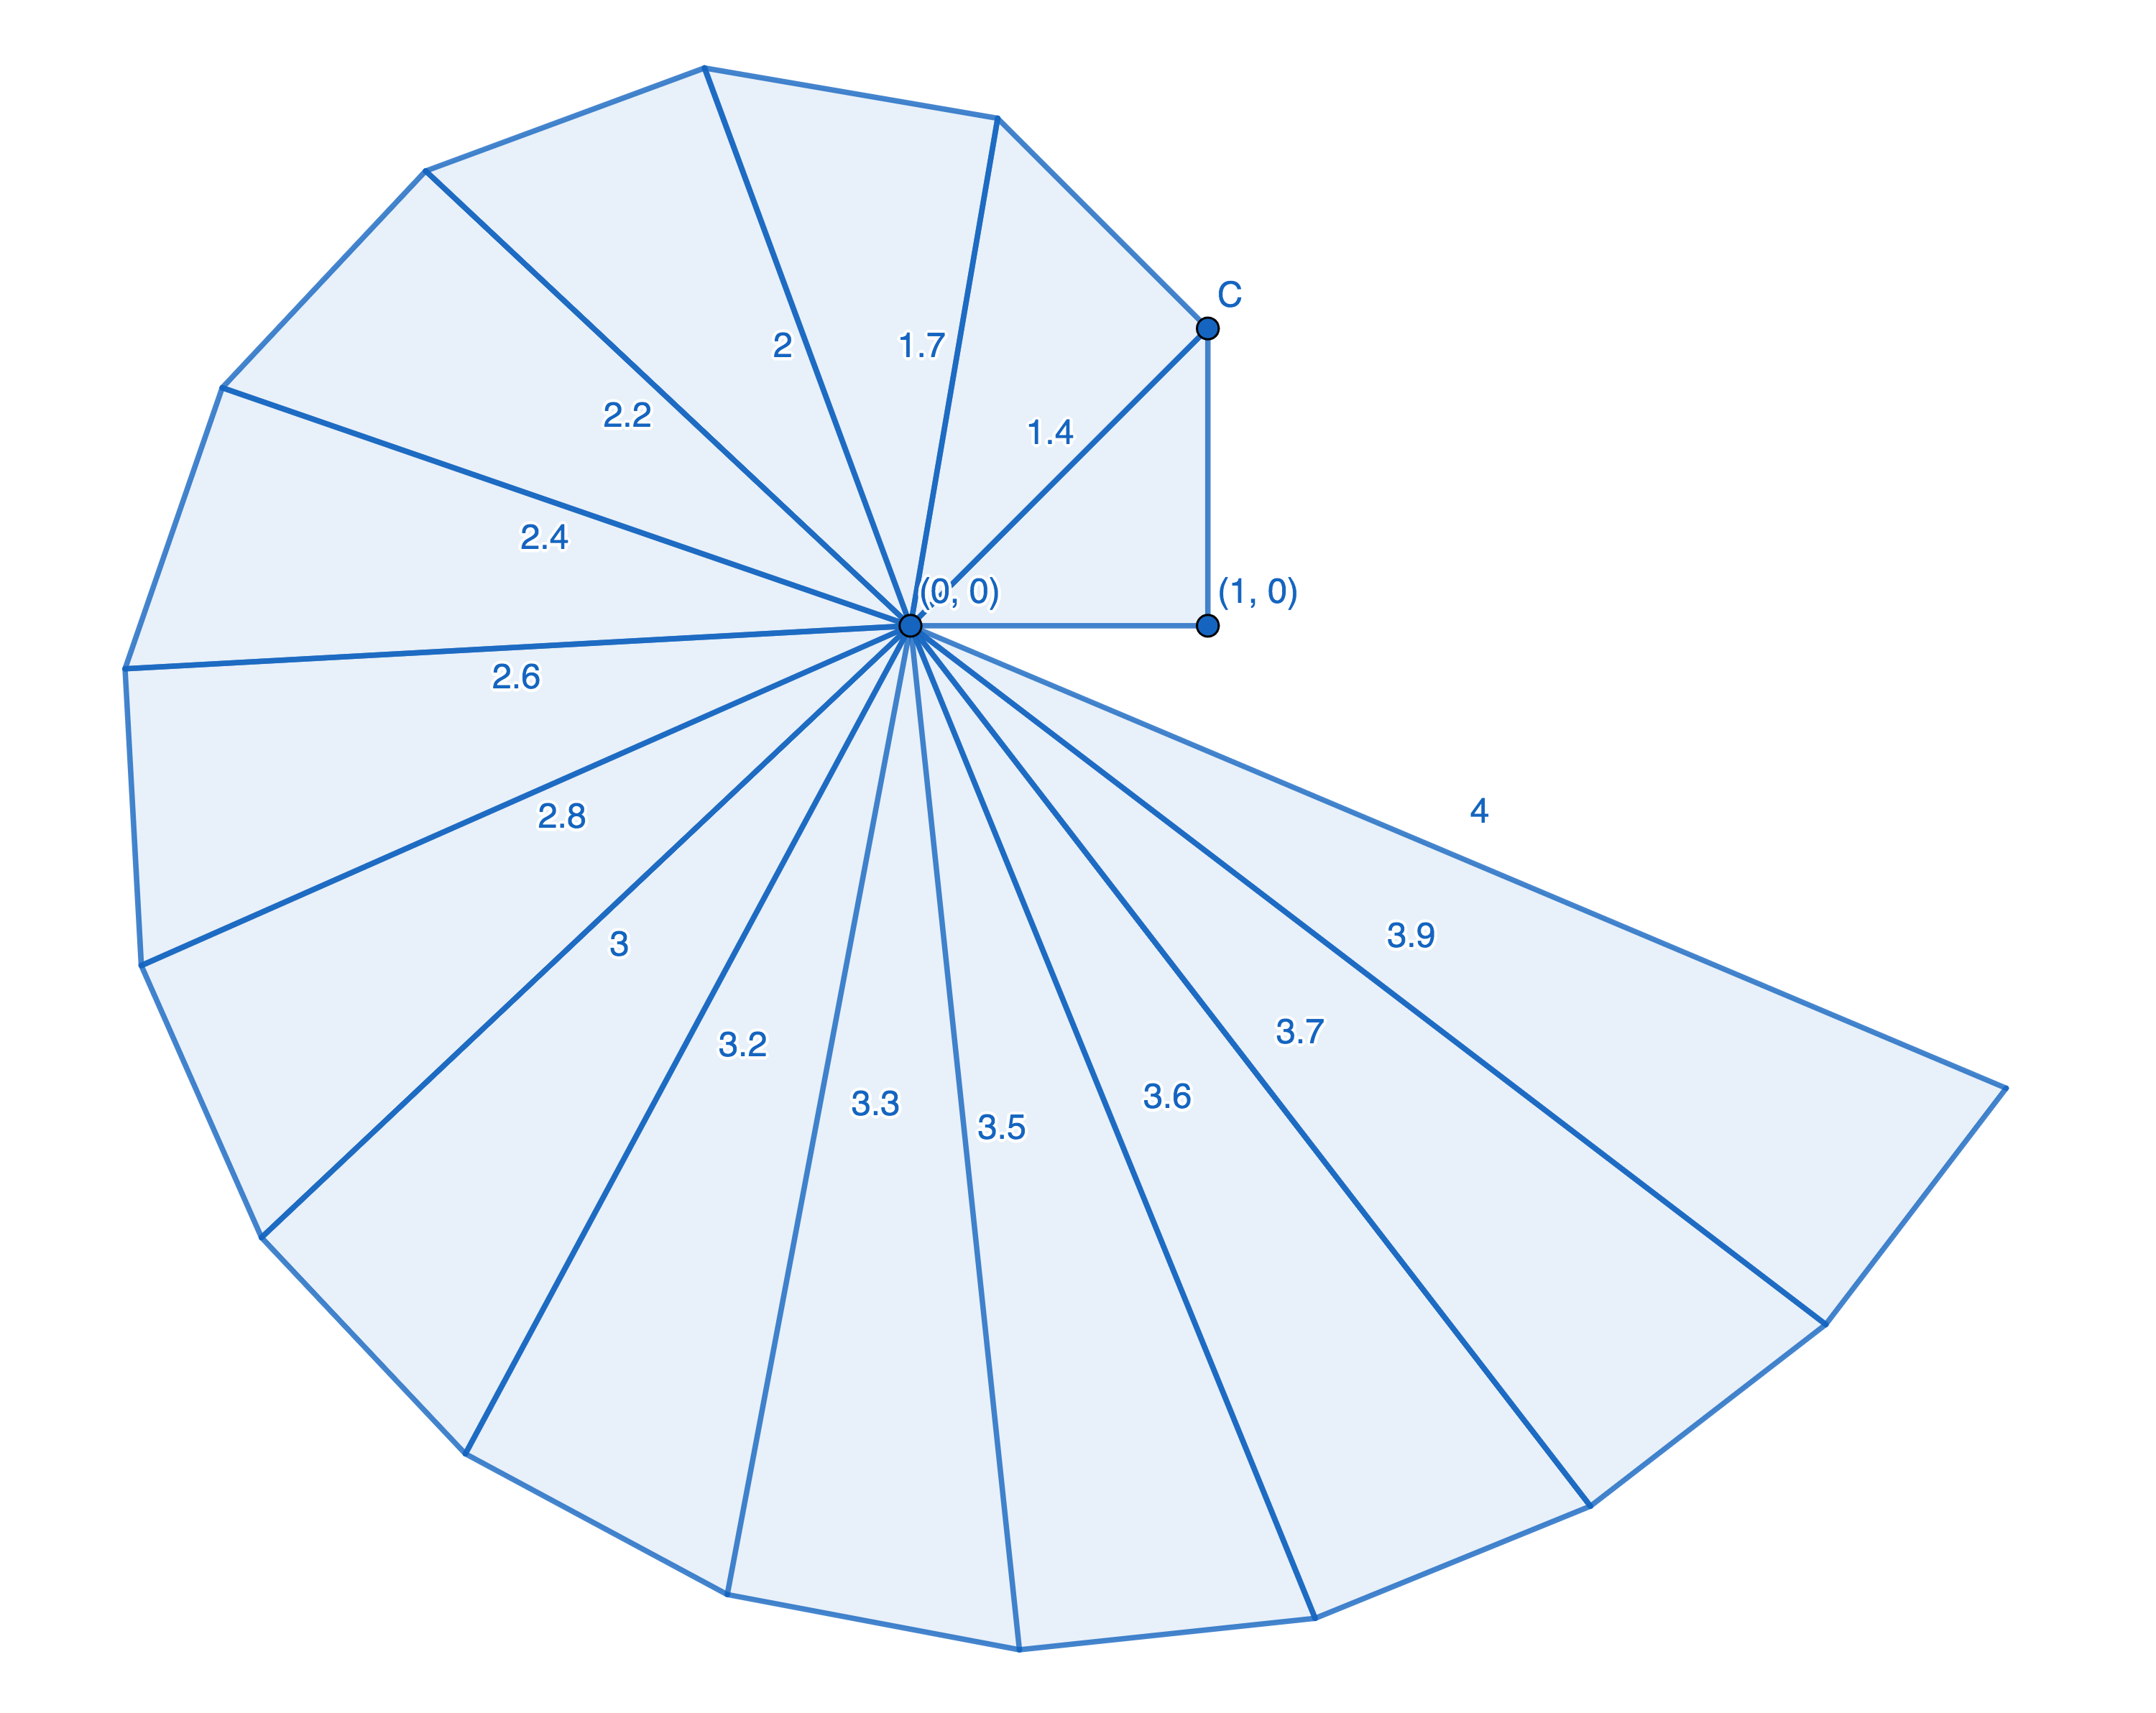
\includegraphics[width=5cm]{6-5CW_Radical-spiral.png}
    \item Briefly explain how the spiral is constructed in the text.
  \end{enumerate}
  \end{block}
  Lesson: Drawing perpendicular figures in Geogebra\\[0.25cm]
  Homework: Complete the project paper (due 10:00pm)
  }

  \section{6.5 Re-Assessment: distance formula, Tuesday 3 December}
  \frame
  {
    \frametitle{Assessment: Distance formula (on looseleaf paper)}
    %\framesubtitle{CCSS: HSG.GPE Express geometric properties with equations \hfill \alert{6.4 Monday 2 Dec}}
    \begin{enumerate}
      \item Find $AB$, $A(-5,1)$ and $B(2,1)$. \hspace{0.5cm}
        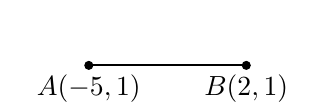
\begin{tikzpicture}[scale=1]
          \draw [thick] (0, 0)--(2,0);
          \draw [fill] (0,0) circle [radius=0.05] node[below]{$A(-5,1)$};
          \draw [fill] (2,0) circle [radius=0.05] node[below]{$B(2,1)$};
        \end{tikzpicture} \vspace{1cm}
      \item Find $c$. \hspace{2cm}
        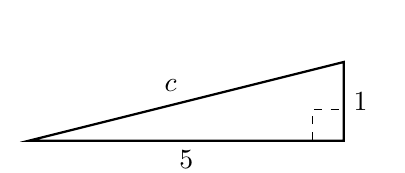
\begin{tikzpicture}[scale=1]
          \node at (2,0.5)[above left]{$c$};
          \node at (4,0.5)[right]{1};
          \node at (2,0)[below]{5};
          \draw [thick] (0, 0)--(4, 0)--(4, 1)--cycle;
          \draw [dashed] (4,0)++(-0.4,0)-- ++(0,0.4)-- +(0.4,0);
        \end{tikzpicture} \vspace{0.5cm}
      \item What is the length of $\overline{CD}$ if $C(-1,15)$ and $D(4,3)$?\\[0.5cm]
        Use $\displaystyle d=\sqrt{(x_2-x_1)^2+(y_2-y_1)^2}$
    \end{enumerate}
  }

  \section{6.6 Midpoint formula, Wednesday 4 December}
  \frame
  {
    \frametitle{GQ: How do we find the midpoint of a line segment?}
    \framesubtitle{CCSS: HSG.GPE Express geometric properties with equations \hfill \alert{6.6 Wednesday 4 Dec}}

    \begin{block}{Do Now pre-quiz: Distance, slope, Pythagorean formula}
    \begin{enumerate}
      \item Bisecting horizontal and vertical distances
      \item Measure diagonal distances
      \item Right triangle situations
    \end{enumerate}
    \end{block}
    Lesson: Midpoint formula (directed segment \& averaging forms)\\
    Review area and volume \\*[5pt]
    Homework: Khan Academy distance practice
  }

  \section{6.7 Midpoint formula, distance quiz, Thursday 5 December}
  \frame
  {
    \frametitle{GQ: How do we find the midpoint of a line segment?}
    \framesubtitle{CCSS: HSG.GPE Express geometric properties with equations \hfill \alert{6.7 Thursday 5 Dec}}

    \begin{block}{Do Now Quiz: Distance, slope, Pythagorean formula}
    \begin{enumerate}
      \item Bisecting horizontal and vertical distances
      \item Measure diagonal distances
      \item Right triangle situations
    \end{enumerate}
    \end{block}
    Lesson: the midpoint formula practice\\
    Review rounding and decimal places \\*[5pt]
    Homework: Handout midpoint practice
  }

  \section{6.8 Tangent introduction, Euclid's Orchard, Friday 6 December}
  \frame
  {
    \frametitle{GQ: How do we map angles to slope?}
    \framesubtitle{CCSS: HSG.GPE Express geometric properties with equations \hfill \alert{6.8 Friday 6 Dec}}

    \begin{block}{Do Now: Euclid's Orchard}
    \begin{enumerate}
      \item Calculate the slope of triangles in the 1st quadrant
      \item Measure their vertex angle measures in degrees
      \item Make a table of the function mapping angle measure to slope
    \end{enumerate}
    \end{block}
    Lesson: Introduction to the tangent function \\
    Homework: Pre-test (\alert{exam Wednesday})
  }

\end{document}

